%! Author = florian
%! Date = 11.12.22
\section{Evaluation of the Elegant Objects Paradigm}\label{sec:evaluation-of-the-elegant-objects-paradigm}
\subsection{Evaluation of the Principles}\label{subsec:evaluation-of-the-principles}
This section will evaluate some elegant-object principles and describe some shortcomings.

One issue of the no null principle is that the author suggests the usage of empty objects, like a nobody employee, as seen in figure\ \ref{fig:empty-object}.
In the companion blog\footnote{\url{https://www.yegor256.com/2014/05/13/why-null-is-bad.html}}, the author writes how null will lead to slowly dying code instead of failing fast.
He neglects that using these empty objects can lead to slowly dying code.
It appears that an operation was successful, but calling specific methods on the empty object will result in an exception.
If null is not an acceptable return value, it should result in an exception and not return an empty object.
Otherwise, this pattern will result in code that checks if an object is the same as an empty object.
In other words, more complicated null checks.

\begin{figure}[h]
    \caption{Empty Object}
    \lstinputlisting[language=Java,basicstyle=\tiny,label={lst:empty-object}]{assets/code/Employee.java}\label{fig:empty-object}
\end{figure}

Another questionable principle is described in subsection\ \ref{subsec:no-instanceof-type-casting-or-reflection}.
The author writes in this blog post\footnote{\url{https://www.yegor256.com/2015/04/02/class-casting-is-anti-pattern.html}} that type casting is an antipattern.
The author means that up-casting is an antipattern, as down-casting is required for some of his examples to work.
In Java, in order to not throw an error, an explicit up-cast is required, as can be seen in figure\ \ref{fig:up-and-down-casting}.

\begin{figure}[h]
    \caption{Up and down casting}
    \lstinputlisting[language=Java,basicstyle=\tiny,label={lst:up-and-down-casting},firstline=3, lastline=4]{assets/code/Casting.java}
    \label{fig:up-and-down-casting}
\end{figure}

The subsection\ \ref{subsec:no-statements-in-test-methods-except-assertthat} explains how using only a single statement in unit tests makes them reusable.
The problem with this is that it only works if classes implement a similar, the same interface or have similar functionality.
Even then, the unit tests often cannot be reused, as there are differences in constructors, for example.
Adhering to an interface and only testing the methods of an interface makes a unit test reusable.
If the interface of two objects is similar enough, the unit tests can be reused.
This can be seen in figure\ \ref{fig:reused-unit-tests}.
Writing only one statement in a unit test can also negatively impact readability.
For example, figure\ \ref{fig:multiple-statements-can-throw} shows a test with multiple method calls in the assert statement.
It needs to be clarified which statement can throw an exception if all calls are in the assert statement.
If the only call that can throw an exception were isolated, it would be easier to read and understand.

\begin{figure}[h]
    \caption{Reusing Unit Tests}
    \lstinputlisting[language=Java,basicstyle=\tiny,label={lst:leftpadded},firstline=20, lastline=24]{../../test/java/at/fhooe/strings/LeftPaddedStringTest.java}
    \lstinputlisting[language=Java,basicstyle=\tiny,label={lst:rightpadded},firstline=19, lastline=23]{../../test/java/at/fhooe/strings/RightPaddedStringTest.java}
    \label{fig:reused-unit-tests}
\end{figure}

\begin{figure}[h]
    \caption{Multiple Statements that can throw}
    \lstinputlisting[language=Java,basicstyle=\tiny,label={lst:multiple-statements-can-throw},firstline=22, lastline=30]{../../test/java/at/fhooe/collections/SplicedListTest.java}
    \label{fig:multiple-statements-can-throw}
\end{figure}

\subsection{Evaluation of the Prototype}\label{subsec:evaluation-of-the-prototype}
The prototype implements the following components:
\begin{itemize}
    \item ArrayList
    \item IntegerRange
    \item EventBus
    \item String utils
\end{itemize}
The prototype adheres to the elegant-object principles as described in section\ \ref{sec:principles}.
The complete source code can be found at \url{https://github.com/flohero/elegant-objects}.

The string utils contains several classes, which simplify working with strings in Java.
They implement the same functionality as the Google Guava Strings class\footnote{\url{https://guava.dev/releases/19.0/api/docs/com/google/common/base/Strings.html}}.
A significant difference between Guava and this implementation is that Guava uses static methods, while the prototype uses only objects since the Elegant Objects principles do not allow static methods, as described in subsection\ \ref{subsec:no-static-methods}.
Most classes do not need a dedicated interface since they only depend on the \texttt{toString}-method.
The tests are short and can be reused for classes with similar functionality, and since nearly all string classes depend on the \texttt{toString}-method, the tests are also similarly structured.

The immutable \texttt{ArrayList} implementations needed several workarounds to work with Elegant Objects.
Since Elegant Objects uses only immutable objects and the iterator interface is inherently mutable, an adapter has to be implemented to restrict mutable code to specific classes.
Figure\ \ref{fig:arraylist-class-diagram} shows the class diagram of the \texttt{ArrayList}.

\begin{figure}[h]
    \caption{Class Diagram of ArrayList}
    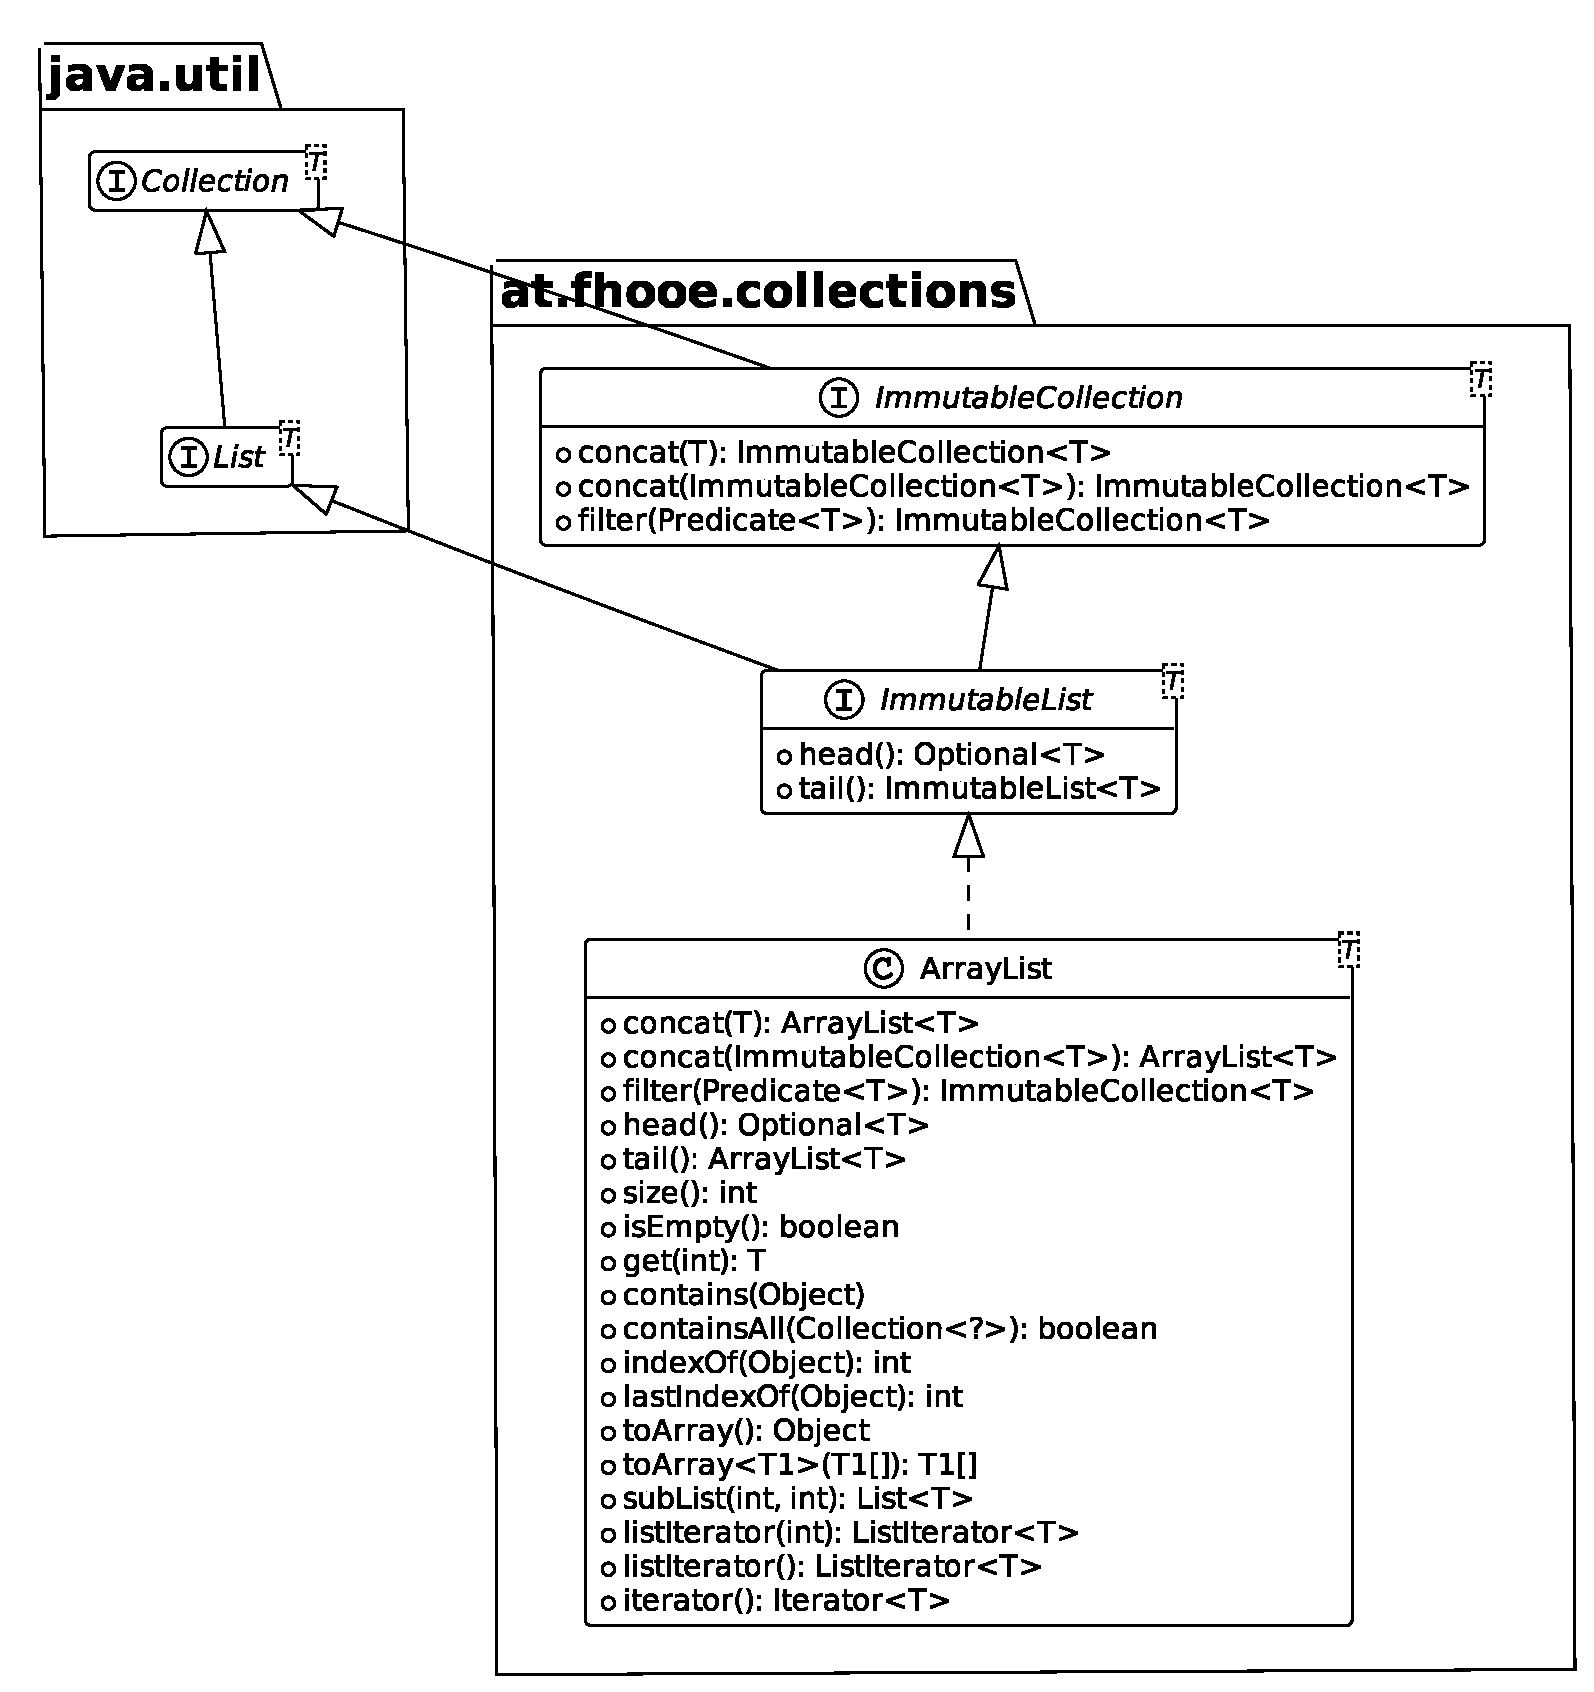
\includegraphics[scale=0.25]{assets/uml/ArrayList-0}
    \label{fig:arraylist-class-diagram}
\end{figure}

\subsection{Developer Experience}\label{subsec:developer-experience}
This subsection describes the developer experience of Elegant Objects.
Adhering to the elegant-object principles will give the resulting objects a more concise and clearly defined interface.
It also results in code that respects the SOLID principles, making a codebase more maintainable and extensible.

The biggest drawback of using Elegant Objects with Java is that Java depends heavily on mutable objects.
Therefore, developers using Elegant Objects have to implement workarounds to limit code where mutable objects are used.
For example, the \texttt{Iterator}-interface\footnote{\url{https://docs.oracle.com/en/java/javase/17/docs/api/java.base/java/util/Iterator.html}}, as seen in figure\ \ref{fig:iterator}, is, per definition, mutable.
The \texttt{next}-method returns the next element in the iteration.
This means an iterator has to depend on an internal state that changes each iteration.
For the sake of using only elegant-object principles where ever possible, an immutable iterator is used, which can be adapted to a Java iterator.
This decision required additional work and implementing an adapter only to meet the elegant-object principles.
It also limited all mutable code to only a few classes, which made the rest easier to test and read.
In the end, the restriction of mutable objects to specific classes increased the readability of the codebase.
Developers can be sure that if an object is successfully constructed, its state is valid.

\begin{figure}[h]
    \caption{Iterator Interface}
    \lstinputlisting[language=Java,basicstyle=\tiny,label={lst:iterator}]{assets/code/Iterator.java}
    \label{fig:iterator}
\end{figure}

Tests become more readable using immutable objects than tests that test mutable objects.
The state of an object can be verified since every method call will return a new object.
The tests are easier to read since there is only one assert statement.
It made it clear what part of an object is tested.

\subsection{Conclusion}\label{subsec:conclusion}
The Elegant Objects paradigm has some valuable practices that help structure code more readably.
Developers must not blindly follow these principles and take the principles with a grain of salt.
